\documentclass[11pt]{article}
%Gummi|065|=)

\usepackage{latexsym,amssymb,amsmath,graphicx,epsfig,amsthm}
\graphicspath{ {Documents/ing2famaf} }

\title{\textbf{Storm, un verificador de modelos probabil\'istico moderno}}
\author{Gonzalo Manuel Garc\'ia $^{1}$\\
		Mar\'ia Luc\'ia Pappaterra $^{1}$\\
		Pablo Vannini $^{1}$ \\ \\
		\small{$^{1}$ Facultad de Matem\'atica, F\'isica, Astronom\'ia y Computaci\'on (FaMAF).}\\ \small {Universidad Nacional de C\'ordoba (UNC). C\'ordoba, Argentina} }
\date{}
\begin{document}

\maketitle

%You are now using Gummi 0.6.6. Many new exciting features have been added to the 0.6 series. The document editor is now a tabbed instance, allowing multiple documents to be worked on simultaneously. Using the new projects menu, you can group files together for easy access. 

%Support for two high-level {\LaTeX} building systems, \emph{rubber}\footnote{https://launchpad.net/rubber/} \& \emph{latexmk}\footnote{http://www.phys.psu.edu/{\textasciitilde}collins/software/latexmk-jcc/} has been added as well. Your preferred typesetter can be configured through the Compilation tab in the Preferences menu. Typesetters that are not installed on your system will not be selectable. 

%Added for your viewing convenience is a continuous preview mode for the PDF. This mode is enabled by default, but can also be disabled through the \emph{(View $\rightarrow$ Page layout in preview)} menu. Complementary to this feature is SyncTeX integration, which allows you to synchronize the position in your editor with the PDF preview. 

%We hope you will enjoy using this release as much as we enjoyed creating it. If you have comments, suggestions or wish to report an issue you are experiencing - contact us at: \emph{https://github.com/alexandervdm/gummi}.

\section{Resumen.}

Los modelos de verificaci\'on probabil\'isticos son fundamentales para el modelado y verificaci\'on de sistemas que exhiben un funcionamiento aleatorio. El presente trabajo es un estudio detallado de la herramienta de verificaci\'on probabil\'istica Storm Checker, a trav\'es de un an\'alisis detallado de los aspectos t\'ecnicos m\'as relevantes de la misma y de la realizaci\'on de un caso de estudio elegido, identificaremos las caracter\'isticas m\'as significativas de la herramienta y la importancia de esta en el campo de la verificaci\'on de sistemas.

\section{Introducci\'on.}

La verificaci\'on de modelos (o model checking) consiste en m\'etodos autom\'aticos de comprobaci\'on de un sistema formal. Dado el modelo de un sistema, en la mayor\'ia de las ocasiones derivado del hardware o del software de un sistema inform\'atico, se comprueba exhaustiva y autom\'aticamente si este modelo cumple con una especificaci\'on dada. El modelo suele estar representado como un sistema de transiciones, es decir, un grafo dirigido, que consta de un conjunto de v\'ertices y aristas, donde un conjunto de proposiciones at\'omicas se asocia a cada nodo. As\'i pues, los nodos representan los estados posibles de un sistema, las aristas posibles evoluciones del mismo, mediante ejecuciones permitidas, que alteran el estado, mientras que las proposiciones representan las propiedades b\'asicas que se satisfacen en cada punto de la ejecuci\'on. Esta representaci\'on se conoce como sistema de transici\'on etiquetado (LTS). La especificaci\'on que debe verificar el modelo contiene requisitos de seguridad tales como la ausencia de bloqueos mutuos (deadlocks) y estados cr\'iticos similares que pueden causar la falla del sistema, la misma es formalmente descrita mediante una f\'ormula, a menudo escrita en alguna variedad de l\'ogica temporal (por ejemplo LTL). Si la especificaci\'on requerida no se verifica, usualmente los programas de verificaci\'on de modelos, devuelven la traza que lleva a la falla en el sistema. En conclusi\'on, la verificaci\'on de modelos comprende las t\'ecnicas para verificar autom\'aticamente las propiedades de correcci\'on de sistemas de estados finitos.

Un modelo de verificaci\'on probabil\'istico es un tipo de verificador (model checker) con ciertas particularidades, en lugar de representar al sistema mediante una m\'aquina de estados finitos, lo hace a trav\'es de un aut\'omata probabil\'istico, que puede ser definido, utilizando cadenas de Marcov. Adem\'as, las especificaciones a verificar deben ser descriptas en alg\'un tipo de l\'ogica temporal probabil\'istica (por ejemplo PCTL). Por \'ultimo, el modelo de verificaci\'on probabil\'istico no devuelve trazas de errores, sino resultados cuantitativos.

Este tipo de verificadores se emplean principalmente para analizar sistemas aleatorios o con fen\'omenos probabil\'isticos. Algunas \'areas y ejemplos de aplicaci\'on son: 

\begin{itemize}
	\item en modelado de incertidumbre y rendimiento, por ejemplo tasas de fallas en protocolos de comunicaci\'on, tiempo de vida de los componentes de un cluster de red, tiempos de llegadas en un sistema de colas, tasas de reacci\'on bioqu\'imica;
	
	\item aleatorizaci\'on utilizada en algoritmos distribuidos para la interrupci\'on de la simetr\'ia entre procesos (por ejemplo: Bluetooth, FireWire);
	
	\item en seguridad inform\'atica, para la generaci\'on de claves aleatorias;
	
	\item en sistemas biol\'ogicos, para modelos de especies o moleculas interactuando alatoriamente dependiendo de su concentraci\'on;
	
	\item en sistemas embebidos, para analizar las fallas de hardware.
\end{itemize} 

Los requisitos son tanto cuantitativos como cualitativos, por ejemplo: en lo referente a la calidad de un servicio: \textquestiondown qu\'e tan confiable es la red Bluetooth de mi autom\'ovil?, \textquestiondown qu\'e tan eficiente es la pol\'itica de administraci\'on de energ\'ia de mi tel\'efono?; otros ejemplos son la cuantificaci\'on de confianza, o del anonimato.

El presente trabajo es un estudio detallado de la herramienta de verificaci\'on probabil\'istica Storm checker. Lo que sigue del art\'iculo esta estructurado de la siguiente manera: a continuaci\'on presentaremos el contexto de creaci\'on de la herramienta, sus principales objetivos y su empleo a nivel usuario. Luego describiremos los aspectos t\'ecnicos m\'as relevantes, como el empleo de cadenas de markov discretas, etc. Finalmente presentaremos los casos de estudios m\'as significativos y el caso de estudio a desarrollar, para finalmente concluir sobre la importancia de Storm en la verificaci\'on de sistemas que dependen de eventos aleatorios. 

\section{Contexto de creaci\'on de la herramienta, objetivos y usuarios de la misma.} 

Storm fue desarrollado en la Universidad de RWTH Aachen, Alemania en el a\~no 2012 por Joost-Pieter Katoen y un grupo de estudiantes de doctorado a su cargo. En la d\'ecada anterior se generaron y mejoraron las herramientas probabil\'isticas de chequeo de modelos, en este contexto Storm se propuso como una plataforma de uso f\'acil para experimentar con nuevos algoritmos de verificaci\'on, modelos probabil\'isticamente ricos, algoritmos mejorados y diferentes formalismos de modelado. Actualmente la herramienta se utiliza tanto en la academia, (ya sea en la misma universidad donde se desarroll\'o, academias independientes o contratadas por la industria), como en la industria propiamente dicha. 

\section{Descripci\'on de la herramienta del lado del usuario.}

HACER

\section{Aspectos t\'ecnicos de la herramienta.}

Storm se basa en modelos de Markov discretos y de tiempo continuo, se centra en las consultas de accesibilidad y su soporte incluye PCTL, CSL, recompensas esperadas y probabilidades condicionales. Tambi\'en ofrece soporte para varios lenguajes de especificaci\'on, entre ellos: PRISM, JANI, GSPNs, DFTs, cpGCL.

\textbf{Cadenas de Markov de tiempo discreto (DTMCs).} Una DTMC es un sistema de transici\'on de estados aumentados con probabilidades. Consiste en un conjunto discreto de estados que representan posibles configuraciones del sistema donde ocurren transiciones entre estados en pasos de tiempo discretos y la probabilidad de hacer transiciones entre estados est\'a dada por distribuciones discretas de probabilidad.
 
Formalmente, una DTMC $D$ es una tupla $(S, s_0, P, L)$, donde $S$ es un conjunto finito de estados, $s_0 \in S$ es el estado inicial. $P: S \times S \rightarrow [0,1]$ es la matriz de probabilidad de transici\'on, donde $\forall  s' \in S$:
\[
\sum_{s' \in S} P(s,s') = 1
\]

y $L: S \rightarrow 2^{AP}$ etiqueta los estados con proposiciones at\'omicas.

En la Figura 1 se presenta un ejemplo de DTMC.

\begin{figure}[h]
	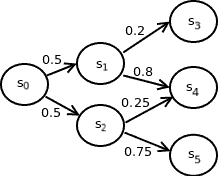
\includegraphics[scale=0.8]{markovchain2.png}
	\centering
	\caption{DTMC}
\end{figure}

\textbf{Procesos de decisi\'on de Markov (MDPs).}

Se trata de una extensi\'on de las DTMCs que permite una elecci\'on no determinista.

\textbf{Cadenas de Markov de tiempo continuo.}

\textbf{Automata de Markov.}

\textbf{Especificaci\'on de propiedades.} La l\'ogica PCTL. Propiedades cuantitativas.

\section{Casos de estudio}

A continuaci\'on desarrollamos brevemente algunos casos de estudio m\'as importantes de la herramienta.

\paragraph{Ajustes finamente automatizados de Algoritmos probabil\'isticamente autoestables.} 

Se trata de un proyecto conjunto de Canad\'a y Alemania, en el cual se estudiaron tres diferentes t\'ecnicas para encontrar la distribuci\'on de probabilidad que logr\'a el m\'inimo tiempo promedio de recuperaci\'on para un input de un protocolo randomizado, distribuido y autoestable sin que modifique el comportamiento del algoritmo. Una de las tres t\'ecnicas consist\'ia en usar Storm para la ``sintes\'is del par\'ametro", donde Storm computa la funci\'on racional, describiendo el tiempo promedio de recuperaci\'on y luego usa 'solvers' (solucionadores) para encontrar el par\'ametro \'optimo de valuaci\'on. Se evaluaron las t\'ecnicas con el algoritmo de 'Herman' (Randomized token circulation) y se obtuvo que la t\'ecnica que utilizaba Storm fue la segunda mas r\'apida.

\paragraph{Verificaci\'on de modelos para el Dise\~no de Protocolos Ultra Confiables para Redes Inal\'ambricas de baja latencia.}

Consiste en una t\'ecnica desarrollada en Suecia en conjunto con Alemania, para dise\~nar protocolos para aplicaciones de seguridad cr\'itica. Tradicionalmente el desarrollo de sistemas inal\'ambricos de baja latencia se baso en simulaciones para identificar arquitecturas viables, la propuesta consisti\'o en usar Storm como herramienta de verificaci\'on probabil\'istica de modelos, para evaluar diferentes variantes de sistemas en la etapa de dise\~no, con la finalidad de proveer l\'imites en %la fiabilidad ??? de ??? 
los dise\~nos a considerar. Se comprob\'o mediante el protocolo de EchoRing, pensado especialmente para aplicaciones industriales de seguridad cr\'itica y basado en sistemas de Tokens, que Storm es una potencial herramienta para la evaluaci\'on de los diferentes dise\~nos de mecanismos para el manejo de un token perdido.

\paragraph{Contraejemplos para recompensas esperadas o costos esperados.}

Se trata de un estudio desarrollado en Alemania con el prop\'osito de demostrar que al emplear Storm como herramienta para la computaci\'on de contraejemplos en sistemas probabil\'isticos para ``recompezas esperadas o costos esperados", se puede obtener un subsistema minimial que ya lleva el costo o la recompenza m\'as alla del l\'imite permitido.

\paragraph{Verificaci\'on de Modelos limitados a programas probabil\'isticos.}

Estados Unidos junto con Alemania investigaron la aplicaci\'on de los enfoques de la verificaci\'on estandar de modelos para verificar propiedades en programas probabil\'isticos. Como el modelo operacional de los programas probabil\'isticos estandar es un proceso potencial param\'etrico infinito de Markov, 
es imposible de una adaptaci\'on directa, % qué significa esto?? 
por lo tanto se propuso un enfoque donde el modelo operacional es creado exitosamente y verificado paso a paso mediante una ejecuci\'on del programa. La evaluaci\'on de dicho modelo es corroborado mediante benchmarks y utilizando Storm para la s\'intesis de par\'ametros.

\paragraph{Modelo basado en el an\'alisis de seguridad para sistema de gu\'ia para veh\'iculos.}

Este caso de estudio es el que hemos elegido para exponer en mayor profundidad. HACER.

\section{Comparaci\'on con otras herramientas.}

Otros model checkers probabil\'isticos: PRISM (utiliza DTMCs, MDPs, CTMCs), ETMCC/MRMC (utiliza DTMCs, CTMCs), LiQuor (verificaci\'on LTL para MDPs), RAPTURE (prototipo para la abstracci\'on / refinamiento de MDPs). Model checkers probabil\'isticos basados en simulaci\'on: APMC, Ymer, VESTA; de comprobaci\'on de CSL para CTMCs: APNN-Toolbox, SMART; para m\'ultiples formalismos: CADP, M\"{o}bius.

\section{Conclusiones.}

\begin{thebibliography}{99}
	\bibitem{Majdi} Majdi Ghadhab, Sebastian Junges, Joost-Pieter Katoen, Matthias Kuntz, Matthias Volk. Model-based Safety Analysis for Vehicle Guidance Systems. Proc. of SAFECOMP, Volume 10488 of LNCS, pages 3–19, Springer, 2017.
\end{thebibliography}


\end{document}
